\PassOptionsToPackage{dvipsnames}{xcolor}
\documentclass[10pt, xcolor={usenames, dvipsnames}]{beamer}

\usepackage[scale=2]{ccicons}
\usepackage{graphicx}
\usepackage{booktabs}
\usepackage{gensymb}
\usepackage{multimedia}
\usepackage{hyperref}
\usepackage{txfonts}
\usepackage{caption}
\usepackage{subcaption}
\usepackage{siunitx}
\usepackage{colortbl}
\usepackage{arydshln}

\usepackage[style=authoryear,backend=biber]{biblatex}
\renewcommand*{\nameyeardelim}{\addcomma\addspace}
\addbibresource{bib/abstract.bib}

% Beamer configuration
\usetheme[sectionpage=progressbar, numbering=counter, progressbar=frametitle]{metropolis}

\usepackage{xfp}
\usepackage{pgfplots}
\usepackage{pgfplotsthemetol}
\usepackage{tikz}
\usetikzlibrary{automata,positioning,arrows,decorations.pathmorphing,calc,patterns,decorations.markings,decorations.shapes,shapes.geometric,matrix}
\usepgfplotslibrary{groupplots,units}
\pgfplotsset{width=7cm,compat=1.18}

\tikzset{paint/.style={ draw=#1, fill=#1 },
         decorate with/.style=
{decorate,decoration={shape backgrounds,shape=#1,shape size=1mm,shape sep=.5cm}}}

% Plot style
\pgfplotsset{
    mplot/.style={
        width=.48\textwidth,
        height=.4\textheight,
        grid=major,
        grid style={dashed,gray!30},
        ylabel style={align=center, font=\bfseries\boldmath},
        xlabel style={align=center, font=\bfseries\boldmath},
        x tick label style={font=\bfseries\boldmath},
        y tick label style={font=\bfseries\boldmath},
        scaled ticks=false,
        label style={font=\footnotesize},
        xticklabel style={font=\footnotesize},
        yticklabel style={font=\footnotesize},
        every axis plot/.append style={solid,thick},
    },
}

% Progressbar
\setbeamercolor{progress bar}{
    fg=TolLightGreen,
    bg=TolLightGreen!50!black!30
}
\makeatletter
    \setlength{\metropolis@titleseparator@linewidth}{2pt}
    \setlength{\metropolis@progressonsectionpage@linewidth}{2pt}
    \setlength{\metropolis@progressinheadfoot@linewidth}{2pt}
\makeatother

% Footer
\setbeamertemplate{frame footer}{Quentin Brateau, ENSTA Bretagne}

% Block fill
\metroset{block=fill}

% Section pages numbering
\makeatletter
\renewcommand{\metropolis@enablesectionpage}{
  \AtBeginSection{
    \ifbeamer@inframe
      \sectionpage
    \else
      \frame[c,plain]{\sectionpage}
    \fi
  }
}
\metropolis@enablesectionpage
\makeatother

% Title
\title{CSI2023 - Torpedo-like AUV control in constrained environment}
\date{\today}
\author{Quentin Brateau}
\institute{ENSTA Bretagne}

\titlegraphic{
    \centering
    \begin{tabular}{lllll}
        \href{https://www.defense.gouv.fr/aid}{\includegraphics[height=0.6cm]{imgs/logo_aid}} &
        \href{https://www.gdr-robotique.org/}{\includegraphics[height=0.6cm]{imgs/logo_gdr}} &
        \href{https://www.ensta-bretagne.fr/fr/}{\includegraphics[height=0.6cm]{imgs/logo_ensta}} &
        \href{https://labsticc.fr/fr}{\includegraphics[height=0.6cm]{imgs/logo_labsticc}} &
        \href{https://www.ensta-bretagne.fr/robex/}{\includegraphics[height=0.6cm]{imgs/logo_robex}}
    \end{tabular}
}

\addtobeamertemplate{frametitle}{}{%
    \begin{tikzpicture}[remember picture,overlay]
    \node[anchor=north east,yshift=2pt] at (current page.north east) {\includegraphics[height=0.85cm]{imgs/logo_ensta_aid}};
    \end{tikzpicture}
}

\begin{document}

    \maketitle

    \section{Context}

        \subsection{PhD presentation}

            \begin{frame}{PhD presentation}
                \centering
                \begin{minipage}[c]{0.58\textwidth}
                    \begin{block}{Research laboratory}
                        \vspace{0.2cm}
                        \begin{itemize}
                            \item ENSTA Bretagne, UMR 6285, Lab-STICC
                        \end{itemize}
                    \end{block}

                    \begin{block}{Supervisiors}
                        \begin{itemize}
                            \item Luc Jaulin
                            \item Fabrice Le Bars
                        \end{itemize}
                    \end{block}

                    \begin{block}{Funding}
                        \begin{itemize}
                            \item AID funding: Jean-Daniel Masson
                        \end{itemize}
                    \end{block}
                \end{minipage}
                \hfill
                \begin{minipage}[c]{0.4\textwidth}
                    \includegraphics[height=0.7\textheight, trim={24cm 0 16cm 0}, clip]{imgs/ensta.jpg}
                \end{minipage}
            \end{frame}

        \subsection{PhD goal}

            \begin{frame}{PhD goal}
                \begin{minipage}[c]{0.55\textwidth}
                    \begin{block}{AUV}
                        \vspace{0.25cm}
                        \begin{itemize}
                            \item Control of torpedo-like AUV \\ 
                            \item Riptide's micro-uuv
                        \end{itemize}
                    \end{block}
                    \begin{block}{Environment}
                        \begin{itemize}
                            \item Constrained environment \\ 
                            \item Pool, harbor, ...
                        \end{itemize}
                    \end{block}
                    \begin{block}{Goals}
                        \begin{itemize}
                            \item Reactivity \\
                            \item Manoeuvrability
                        \end{itemize}
                    \end{block}
                \end{minipage}
                \hfill
                \begin{minipage}[c]{0.4\textwidth}
                    \begin{figure}[htb]
                        \includegraphics[width=\textwidth]{imgs/harbour.png}

                        \vspace{.1cm}

                        \includegraphics[width=\textwidth]{imgs/Riptide.jpeg}
                        \caption{Harbor and Riptide in the ENSTA Bretagne pool}
                    \end{figure}
                \end{minipage}
            \end{frame}

    \begin{frame}{Table of contents}
        \setbeamertemplate{section in toc}[sections numbered]
        \tableofcontents[hideallsubsections]
    \end{frame}

    \section{Riptide presentation}

        \begin{frame}{Torpedo Model}
            \begin{minipage}[t]{.48\textwidth}
                \begin{block}<+->{Controlled physical quantities}
                    \vspace{2.5mm}
                    \begin{itemize}
                        \item Linear acceleration $\mathbf{a_r}$
                        \item angular velocity $\mathbf{\omega_r}$
                    \end{itemize}
                \end{block}
                \begin{block}<+->{Robot's inputs}
                    \centering
                    Input vector of the system is $\mathbf{u} = (u_0, u_1, u_2, u_3)^T$, where:
                    \begin{itemize}
                        \item $u_0$: thruster velocity \\
                        \item $u_1, u_2, u_3$: fin angles
                    \end{itemize}
                \end{block}
            \end{minipage}
            \hfill
            \begin{minipage}[t]{.48\textwidth}
                \begin{block}<+->{Torpedo velocity}
                    \vspace{2.5mm}
                    \begin{equation}
                        \mathbf{v_r} = (v_r, 0, 0)^T
                    \end{equation}
                \end{block}
                \onslide<+->{
                    \begin{figure}
                        \centering
                        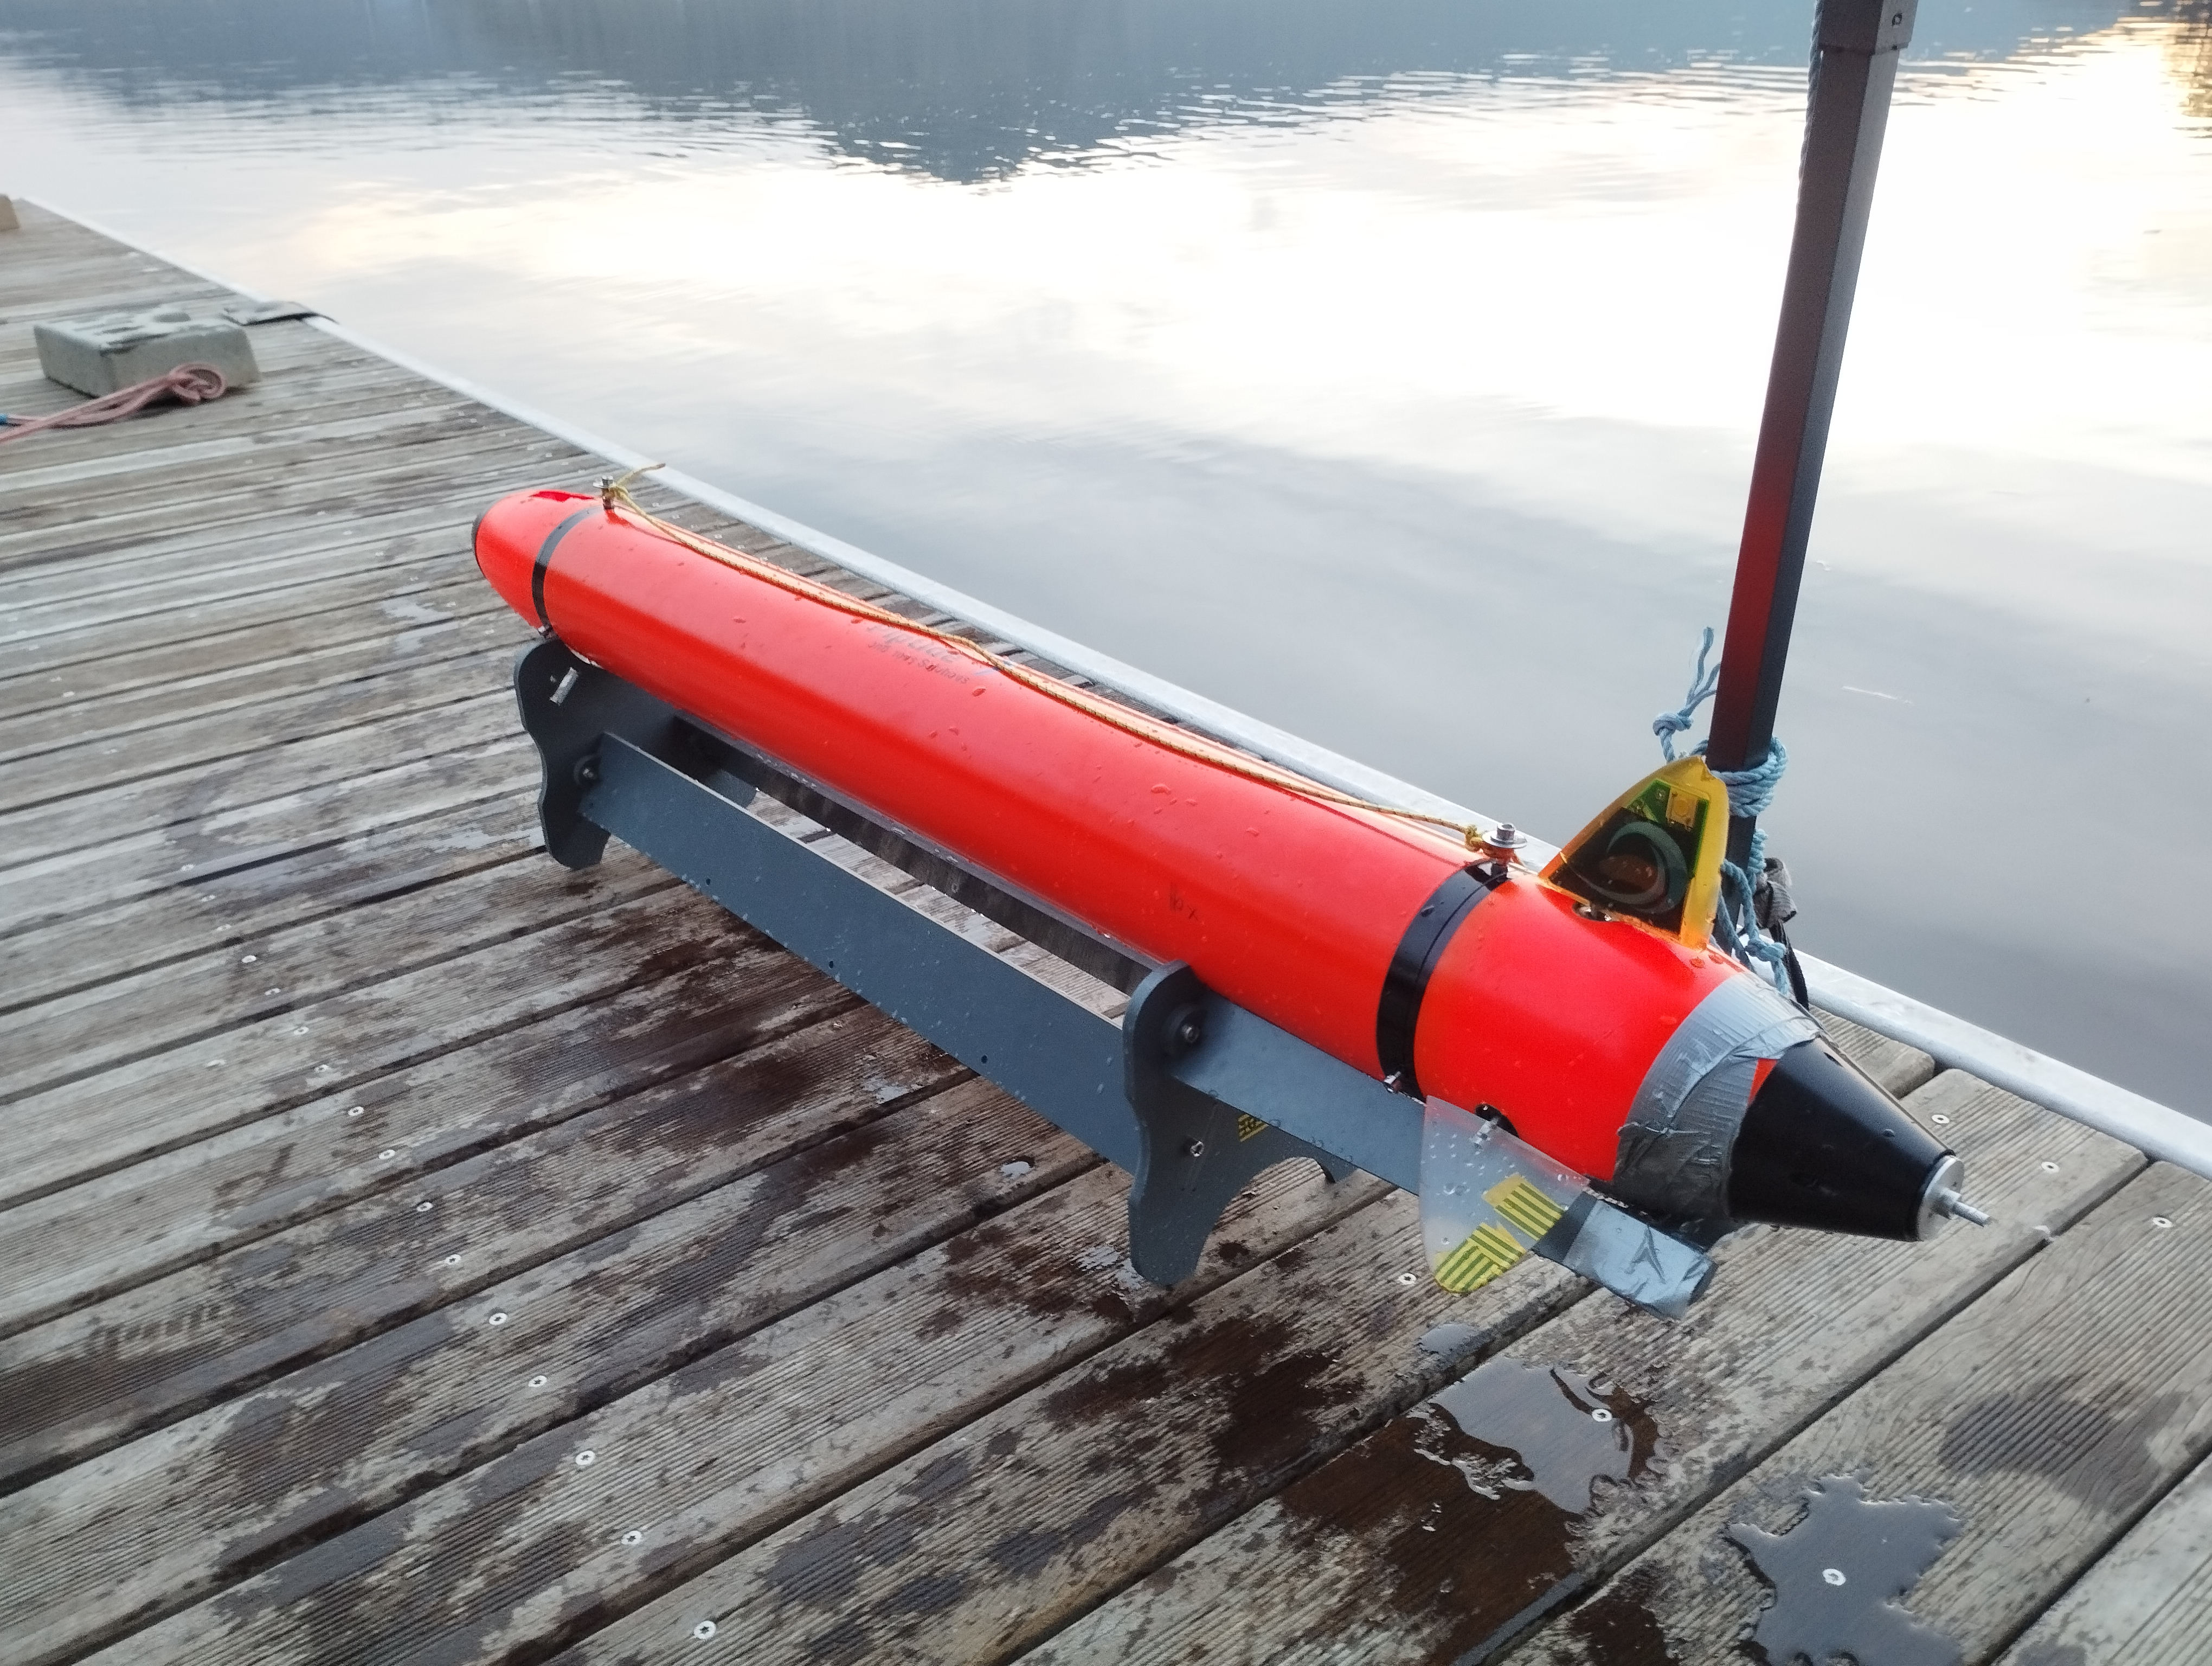
\includegraphics[width=.9\textwidth,trim={0 4cm 0 8cm},clip]{imgs/riptide_pontoon.jpg}
                        \caption{Riptide}
                    \end{figure}
                }
            \end{minipage}
        \end{frame}

        \begin{frame}{Operating systems}
            \begin{figure}
                \begin{subfigure}[c]{.5\textwidth}
                    \includegraphics[width=.95\textwidth]{imgs/simulation.png}
                    \subcaption{Riptide's simulator}
                \end{subfigure}%
                \begin{subfigure}[c]{.5\textwidth}
                    \includegraphics[width=.95\textwidth]{imgs/riptide.png}
                    \subcaption{Riptide robot}
                \end{subfigure}
                \caption{Riptide operating systems}
            \end{figure}
        \end{frame}

    \section{Attitude control for AUV}

        \begin{frame}{Attitude control for AUV}
            \begin{minipage}[c]{0.48\textwidth}
                \begin{block}{Log control}
                    \begin{itemize}
                        \vspace{0.25cm}
                        \item<2-> Simple control law
                        \item<3-> Complete attitude control
                        \item<4-> Fastest reorientation
                        \item<5-> Rigid control
                    \end{itemize}
                \end{block}
            \end{minipage}
            \hfill
            \begin{minipage}[c]{0.48\textwidth}
                \begin{block}{Orthogonal control}
                    \begin{itemize}
                        \vspace{0.25cm}
                        \item<2-> Simple control law
                        \item<3-> Partial attitude control
                        \item<4-> Fastest reorientation
                        \item<5-> Slack Control
                    \end{itemize}
                \end{block}
            \end{minipage}
        \end{frame}

        \subsection{Log Control}

            \begin{frame}{Log control - Illustration}
                \begin{figure}
                    \begin{subfigure}[t]{.5\textwidth}
                        \centering
                        \begin{tikzpicture}[
                            wavy/.style={->,>=latex,thick,decorate,
                            decoration={snake,amplitude=2mm,segment length=8mm,pre length=1mm, post length=1mm}}
                            ]
                            \shade[ball color = gray!40, opacity = 0.4] (0,0) circle (2cm);
                            \draw[thick] (0,0) circle (2cm);
                            \onslide<1->{
                                \begin{scope}
                                    \draw[thick] (-2,0) arc (180:360:2 and 0.6) coordinate[pos=0.3] (R3);
                                    \draw[dashed] (2,0) arc (0:180:2 and 0.6);
                                \end{scope}
                            }
                            \onslide<2->{
                                \coordinate (R1) at (0.8,1.3);
                                \draw[thick,red,->,>=latex] (0,0) -- node[midway,above left] {$\mathbf{u}$} (R1); 
                            }
                            \onslide<3->{
                                \draw[thick,RoyalBlue,->,>=latex] (0,0) -- node[midway,above] {$\mathbf{v}$} (R3);
                            }
                            \coordinate (R4) at (-0.8,1.3);
                            \onslide<4>{
                                \draw[wavy,ForestGreen] (R1) to[bend right=45] (R3);
                                \node[ForestGreen] at (R4) {$\mathbf{w}$};
                            }
                            \onslide<5>{
                                \path[thick,->,>=latex,RoyalPurple] (R1) edge[in=90,out=130] (R3);
                                \node[RoyalPurple] at (R4) {$\mathbf{w}$};
                            }
                        \end{tikzpicture}
                        \subcaption{Representation in $S^2$}
                    \end{subfigure}%
                    \begin{subfigure}[t]{.5\textwidth}
                        \centering
                        \begin{tikzpicture}[
                            wavy/.style={->,>=latex,thick,decorate,
                            decoration={snake,amplitude=2mm,segment length=8mm,pre length=1mm, post length=1mm}}
                            ]
                            \shade[ball color = gray!40, opacity = 0.4] (0,0) circle (2cm);
                            \draw[thick] (0,0) circle (2cm);
                            \onslide<1->{
                                \begin{scope}
                                    \draw[thick] (-2,0) arc (180:360:2 and 0.6) coordinate[pos=0.3] (R3);
                                    \draw[dashed] (2,0) arc (0:180:2 and 0.6);
                                \end{scope}
                            }
                            \onslide<3->{
                                \node[thick,RoyalBlue] at (R3) {$\bullet$} node[RoyalBlue] at (R3) [below] {$\mathbf{R_v}$};
                            }
                            \coordinate (R4) at (-0.8,1.3);
                            \onslide<4>{
                                \draw[wavy,ForestGreen,densely dotted] (R1) to[bend right=45] (R3);
                                \node[ForestGreen] at (R4) {$\mathbf{R_w}$};
                            }
                            \onslide<5->{
                                \path[thick,->,>=latex,RoyalPurple,densely dotted] (R1) edge[in=90,out=130] (R3);
                                \node[RoyalPurple] at (R4) {$\mathbf{R_w}$};
                            }
                            \onslide<2->{
                                \coordinate (R1) at (0.8,1.3);
                                \node[red] at (R1) {$\bullet$} node[red] at (R1) [below right] {$\mathbf{R_u}$};
                            }
                        \end{tikzpicture}
                        \caption{Representation in $SO(3)$}
                    \end{subfigure}
                    \caption{Log control}
                \end{figure}
            \end{frame}

            \begin{frame}{Log control - Formula}
                \centering
                \begin{minipage}{0.5\textwidth}
                    \begin{block}<+->{Rotation matrix}
                        \begin{equation}
                            \mathbf{\color{RoyalPurple}R_w} = \mathbf{\color{red}R_u}^T \cdot \mathbf{\color{RoyalBlue}R_v}
                        \end{equation}
                    \end{block}
                    \begin{block}<+->{Angular velocity w}
                        Link between $\mathbf{\color{RoyalPurple}w}$ and $\mathbf{\color{RoyalPurple}R_w}$.
                        \begin{align}
                            \onslide<+->{\mathbf{\color{RoyalPurple}R_w}^{\color{RubineRed}t} &= Exp~\mathbf{\color{RoyalPurple}w} \\}
                            \onslide<+->{\mathbf{\color{RoyalPurple}w} &= {\color{RubineRed}t} \cdot Log~\mathbf{\color{RoyalPurple}R_w} \\}
                            \notag
                        \end{align}
                        \vskip-1.5em
                    \end{block}
                \end{minipage}%
                \begin{minipage}{0.5\textwidth}
                    \centering
                    \begin{figure}
                        \begin{subfigure}[c]{\textwidth}
                            \centering
                            \begin{tikzpicture}
                                \shade[ball color = gray!40, opacity = 0.4] (0,0) circle (2cm);
                                \draw[thick] (0,0) circle (2cm);
                                \begin{scope}
                                    \draw[thick] (-2,0) arc (180:360:2 and 0.6) coordinate[pos=0.3] (R3);
                                    \draw[dashed] (2,0) arc (0:180:2 and 0.6);
                                \end{scope}
                                \coordinate (R1) at (0.8,1.3);
                                \coordinate (R4) at (-0.8,1.3);
                                \node[thick,RoyalBlue] at (R3) {$\bullet$} node[RoyalBlue] at (R3) [below] {$\mathbf{R_v}$};
                                \path[thick,->,>=latex,RoyalPurple,densely dotted] (R1) edge[in=90,out=130] (R3);
                                \node[RoyalPurple] at (R4) {$\mathbf{R_w}$};
                                \node[red] at (R1) {$\bullet$} node[red] at (R1) [below right] {$\mathbf{R_u}$};
                            \end{tikzpicture}
                            \caption{Representation in $SO(3)$}
                        \end{subfigure}
                        \caption{Log Control}
                    \end{figure}
                \end{minipage}%
            \end{frame}

            \begin{frame}{Log control - Extension}
                \begin{minipage}{.48\textwidth}
                    \begin{block}{2D Extension}
                        \vspace{.25cm}
                        \begin{itemize}[<+->]
                            \item $Log$ of a rotation matrix
                            \item Find sawtooth {\small $sawtooth(x) = 2 \cdot atan\left(tan\left(\frac{x}{2}\right)\right)$}
                        \end{itemize}
                    \end{block}
                    \begin{block}<+->{ND Extension}
                        \begin{itemize}[<+->]
                            \item Control of ND system
                        \end{itemize}
                    \end{block}
                \end{minipage}%
                \hfill
                \begin{minipage}{.5\textwidth}
                    \onslide<2->{
                        \begin{figure}
                            \centering
                            \begin{tikzpicture}
                                \begin{axis}[
                                        mplot, width=.95\textwidth, height=.5\textheight, name=sawtooth,
                                        xlabel=$\theta$, xmin=-6.28318, xmax=6.28318,
                                        xtick={-6.28318, -3.14159, 0, 3.14159, 6.28318},
                                        xticklabels={$-2\pi$, $-\pi$, 0, $\pi$, $2\pi$},
                                        ylabel=$Log(A(\theta))$, ymin=-4, ymax=4,
                                        ytick={-3.14159, 0, 3.14159},
                                        yticklabels={$-\pi$, 0, $\pi$},
                                        domain=-6.28318:6.28318, samples=100,
                                    ]
                                    \addplot[RoyalBlue] {2.*3.1415/180.*atan(tan(x*90/3.1415))};
                                \end{axis}
                            \end{tikzpicture}
                            \caption{$Log$ in $SO(2)$}
                        \end{figure}
                    }
                \end{minipage}
            \end{frame}

        \subsection{Orthogonal Control}

            \begin{frame}{Orthogonal control - Illustration}
                \begin{figure}
                    \begin{subfigure}[c]{.5\textwidth}
                        \centering
                        \begin{tikzpicture}
                            \shade[ball color = gray!40, opacity = 0.4] (0,0) circle (2cm);
                            \draw[thick] (0,0) circle (2cm);
                            \onslide<2->{
                                \coordinate (R1) at (0.8,1.3);
                                \draw[thick,red,->,>=latex] (0,0) -- node[midway,above left] {$\mathbf{u}$} (R1); 
                            }
                            \onslide<3->{
                                \coordinate (R2) at (-0.2,1.15);
                                \draw[thick,ForestGreen,->,>=latex] (0,0) -- node[midway,above left] {$\mathbf{v}$} (R2); 
                            }
                            \onslide<4->{
                                \begin{scope}[rotate around={-30:(0,0)}]
                                    \draw[thick] (-2,0) arc (180:360:2 and 0.6) coordinate[pos=0.36] (R3) coordinate[pos=0.61] (R4);
                                    \draw[dashed] (2,0) arc (0:180:2 and 0.6);
                                \end{scope}
                                \draw[thick,dotted] (R1) edge[in=30,out=175] (R2);
                                \draw[thick,RoyalBlue,->,>=latex] (0,0) -- node[midway,above] {$\mathbf{v_\bot}$} (R3);
                            }
                            \onslide<4>{
                                \draw[thick,dotted] (R2) edge[in=70,out=210] (R3);
                            }
                            \onslide<5->{
                                \path[thick,->,>=latex,RoyalPurple] (R2) edge[in=70,out=210] node[midway,above,left,RoyalPurple] {$\alpha$} (R3);
                                \draw[thick,RoyalPurple,->,>=latex] (0,0) -- node[midway,right] {$\mathbf{w}$} (R4);
                            }
                        \end{tikzpicture}
                        \subcaption{Representation in $S^2$}
                    \end{subfigure}%
                    \begin{subfigure}[c]{.5\textwidth}
                        \centering
                        \begin{tikzpicture}
                            \shade[ball color = gray!40, opacity = 0.4] (0,0) circle (2cm);
                            \draw[thick] (0,0) circle (2cm);
                            \onslide<2->{
                                \coordinate (R1) at (0.8,1.3);
                                \node[red] at (R1) {$\bullet$} node[red] at (R1) [below right] {$\mathbf{R_u}$};
                            }
                            \onslide<3->{
                                \coordinate (R2) at (-0.2,1.15);
                                \node[ForestGreen] at (R2) {$\bullet$} node[ForestGreen] at (R2) [above left] {$\mathbf{R_v}$};
                            }
                            \onslide<4->{
                                \begin{scope}[rotate around={-30:(0,0)}]
                                    \draw[thick] (-2,0) arc (180:360:2 and 0.6) coordinate[pos=0.36] (R3);
                                    \draw[dashed] (2,0) arc (0:180:2 and 0.6);
                                \end{scope}
                                \node[thick,RoyalBlue] at (R3) {$\bullet$} node[RoyalBlue] at (R3) [below left] {$\mathbf{R_{v_\bot}}$};
                            }
                            \onslide<5->{
                                \path[thick,->,>=latex,RoyalPurple,densely dotted] (R2) edge[in=70,out=210] node[midway, left] {$\mathbf{R_w}$} (R3);
                            }
                        \end{tikzpicture}
                        \subcaption{Representation in $SO(3)$}
                    \end{subfigure}
                    \caption{Orthogonal Control}
                \end{figure}
            \end{frame}

            \begin{frame}{Orthogonal Control - Determine $\mathbf{v_\bot}$}
                \begin{minipage}[c]{.4\textwidth}
                    \centering
                    \begin{figure}
                        \begin{tikzpicture}
                            \shade[ball color = gray!40, opacity = 0.4] (0,0) circle (2cm);
                            \draw[thick] (0,0) circle (2cm);
                            \coordinate (R1) at (0.8,1.3);
                            \draw[thick,red,->,>=latex] (0,0) -- node[midway,above left] {$\mathbf{u}$} (R1);
                            \begin{scope}[rotate around={-30:(0,0)}]
                                \draw[thick] (-2,0) arc (180:360:2 and 0.6) coordinate[pos=0.36] (R3);
                                \draw[dashed] (2,0) arc (0:180:2 and 0.6);
                            \end{scope}
    
                            \onslide<1-4> {
                                \coordinate (R2) at (-0.2,1.15);
                                \draw[thick,ForestGreen,->,>=latex] (0,0) -- node[midway,left]  {$\mathbf{v}$} (R2);
                            }
                            
                            \onslide<2> {
                                \coordinate (vu) at ($(0,0)!0.78!(R1)$);
                                \draw[thick,dotted] (vu) -- (R2);
                                \draw[thick,RoyalPurple,->,>=latex] (0,0) -- node[midway,right] {$\langle \mathbf{u}, \mathbf{v}\rangle \cdot \mathbf{u}$} (vu);
                            }
                            \onslide<3> {
                                \coordinate (vv) at ($(0,0)!0.72!(R3)$);
                                \draw[thick,RoyalPurple,->,>=latex] (vv) -- node[midway,left] {$\langle \mathbf{u}, \mathbf{v}\rangle \cdot \mathbf{u}$} (R2);
                                \draw[thick,RoyalBlue,->,>=latex] (0,0) -- node[midway,below right] {$\mathbf{v} - \langle \mathbf{u}, \mathbf{v}\rangle \cdot \mathbf{u}$} (vv);
                                }
                            \onslide<4> {
                                \draw[thick,RoyalBlue,->,>=latex] (0,0) -- node[midway,below right] {$\mathbf{v_\bot}$} (R3);
                            }
    
                            \onslide<5> {
                                \draw[thick,ForestGreen,->,>=latex] (0,0) -- node[midway,right] {$\mathbf{v}$} (R1);
                            }
                        \end{tikzpicture}
                        \caption{Representation in $S^2$}
                    \end{figure}
                \end{minipage}%
                \hfill
                \begin{minipage}[c]{.55\textwidth}
                    \vfill
                    \begin{block}{Determine $\mathbf{v_\bot}$}
                        \begin{equation}
                            \mathbf{\color{RoyalBlue}{v_\bot}} = \frac{\mathbf{\color{ForestGreen}{v}} - \langle \mathbf{\color{red}{u}}, \mathbf{\color{ForestGreen}{v}}\rangle \cdot \mathbf{\color{red}{u}}}{||\mathbf{\color{ForestGreen}{v}} - \langle \mathbf{\color{red}{u}}, \mathbf{\color{ForestGreen}{v}}\rangle \cdot \mathbf{\color{red}{u}}||}
                        \end{equation}
                    \end{block}
                    \begin{block}<5->{Limitation}
                        Physical singularity when $\mathbf{\color{red}{u}} = \mathbf{\color{ForestGreen}{v}}$, as $\mathbf{\color{RoyalBlue}{v_\bot}}$ is undefined
                    \end{block}
                    \vfill
                \end{minipage}
            \end{frame}

            \begin{frame}{Orthogonal Control - Determine $\mathbf{\omega}$}
                \begin{minipage}[c]{.4\textwidth}
                    \centering
                    \begin{figure}
                        \begin{tikzpicture}
                            \shade[ball color = gray!40, opacity = 0.4] (0,0) circle (2cm);
                            \draw[thick] (0,0) circle (2cm);
                            \coordinate (R1) at (0.8,1.3);
                            \draw[thick,red,->,>=latex] (0,0) -- node[midway,above left] {$\mathbf{u}$} (R1);
                            \draw[thick,RoyalBlue,->,>=latex] (0,0) -- node[midway,above] {$\mathbf{v_\bot}$} (R3);
                            \begin{scope}[rotate around={-30:(0,0)}]
                                \draw[thick] (-2,0) arc (180:360:2 and 0.6) coordinate[pos=0.36] (R3) coordinate[pos=0.61] (R4);
                                \draw[dashed] (2,0) arc (0:180:2 and 0.6)  coordinate[pos=0.36] (R5);
                            \end{scope}
                            
                            \onslide<1>{
                                \coordinate (R2) at (-0.2,1.15);
                                \draw[thick,ForestGreen,->,>=latex] (0,0) -- node[midway,above left] {$\mathbf{v}$} (R2); 
                                \draw[thick,dotted] (R1) edge[in=30,out=175] (R2);
                                \draw[thick,dotted] (R2) edge[in=70,out=210] (R3);
                            }
    
                            \onslide<2>{
                                \draw[thick,ForestGreen,->,>=latex] (0,0) -- node[midway,below right] {$\mathbf{v}$} (R3);
                            }
    
                            \onslide<3>{
                                \draw[thick,ForestGreen,->,>=latex] (0,0) -- node[midway,below right] {$\mathbf{v}$} (R5);
                            }
                        \end{tikzpicture}
                        \caption{Representation in $S^2$}
                    \end{figure}
                \end{minipage}
                \hfill
                \begin{minipage}[c]{.55\textwidth}
                    \vfill
                    \begin{block}{Rotation matrix}
                        \begin{equation}
                            \begin{array}{rcl}
                                \mathbf{K}_{\mathbf{\color{ForestGreen}{v}}}^{\mathbf{\color{RoyalBlue}{v_\bot}}} & = & \mathbf{\color{RoyalBlue}{v_\bot}} \mathbf{\color{ForestGreen}{v}}^T - \mathbf{\color{ForestGreen}{v}}\mathbf{\color{RoyalBlue}{v_\bot}}^T \\
                                \mathbf{R}_{\mathbf{\color{ForestGreen}{v}}}^{\mathbf{\color{RoyalBlue}{v_\bot}}} & = & \mathbf{I_3} + \mathbf{K}_{\mathbf{\color{ForestGreen}{v}}}^{\mathbf{\color{RoyalBlue}{v_\bot}}} + \frac{1}{1 + \color<3>{red}{\langle \mathbf{\color<-2>{ForestGreen}{v}}, \mathbf{\color<-2>{RoyalBlue}{v_\bot}}\rangle}} (\mathbf{K}_{\mathbf{\color{ForestGreen}{v}}}^{\mathbf{\color{RoyalBlue}{v_\bot}}})^2 \\
                            \end{array}
                        \end{equation}
                    \end{block}
                    \begin{block}<2->{No singularities}
                        \vspace{.2cm}
                        \begin{itemize}
                            \item If $\mathbf{\color{ForestGreen}{v}} = \mathbf{\color{RoyalBlue}{v_\bot}}$, $\mathbf{K}_{\mathbf{\color{ForestGreen}{v}}}^{\mathbf{\color{RoyalBlue}{v_\bot}}}=\mathbf{O_3}$ and $\mathbf{R_{{\color{ForestGreen}{v}}}^{{\color{RoyalBlue}{v_\bot}}}} = \mathbf{I_3}$ 
                            \item<3> Singularity when $\langle\mathbf{\color{ForestGreen}{v}}, \mathbf{\color{RoyalBlue}{v_\bot}}\rangle = -1$
                        \end{itemize}
                    \end{block}
                    \vfill
                \end{minipage}
            \end{frame}

        \subsection{Approaches comparison}

            \begin{frame}{Approaches comparison}
                \begin{minipage}[t]{0.48\textwidth}
                    \centering
                    \textbf{\large Classical control}
                    \begin{block}<2->{Strengths}
                        \begin{itemize}
                            \item Fully controlled attitude
                        \end{itemize}
                    \end{block}
                    \begin{block}<3->{Weaknesses}
                        \begin{itemize}
                            \item Complete knowledge of $\mathbf{R}$
                            \item Complete attitude setpoint
                            \item Slower reorientation
                        \end{itemize}
                    \end{block}
                \end{minipage}
                \hfill
                \begin{minipage}[t]{0.48\textwidth}
                    \centering
                    \textbf{\large Orthogonal control}
                    \begin{block}<2->{Strengths}
                        \begin{itemize}
                            \item Partial knowledge of $\mathbf{R}$
                            \item Partial attitude control
                            \item Quickest reorientation
                            \item Controllable remaining attitude
                        \end{itemize}
                    \end{block}
                    \begin{block}<3->{Weaknesses}
                        \begin{itemize}
                            \item Uncontrolled direction
                        \end{itemize}
                    \end{block}
                \end{minipage}
            \end{frame}
    
    \section{Trials}

        \subsection{Guerlédan}

            \begin{frame}{Trials}
                \begin{minipage}[c]{.55\textwidth}
                    \begin{block}<+->{2023 - Week 6}
                        \vspace{2.5mm}
                        \begin{itemize}
                            \item Riptide first trial
                            \item Riptide controller
                        \end{itemize}
                    \end{block}
                    \begin{block}<+->{2023 - Week 8}
                        \begin{itemize}
                            \item Riptide hardware fix
                            \item Depth controller
                        \end{itemize}
                    \end{block}
                    \begin{block}<+->{2023 - Week 21}
                        \begin{itemize}
                            \item Riptide hardware test
                            \item Log controller
                        \end{itemize}
                    \end{block}
                \end{minipage}%
                \hfill
                \begin{minipage}[c]{.43\textwidth}
                    \centering
                    \begin{figure}
                        \centering
                        \begin{subfigure}[t]{.9\textwidth}
                            \centering
                            \includegraphics[width=\textwidth,trim={0 1cm 0 0.8cm},clip]{imgs/lac-de-guerledan.jpg}
                            \subcaption{Guerlédan's dam\footnote[frame]{\url{https://www.saint-aignan56.fr/tourisme/lac-de-guerledan/}}}
                        \end{subfigure}
                        \hfill
                        \begin{subfigure}[t]{.9\textwidth}
                            \centering
                            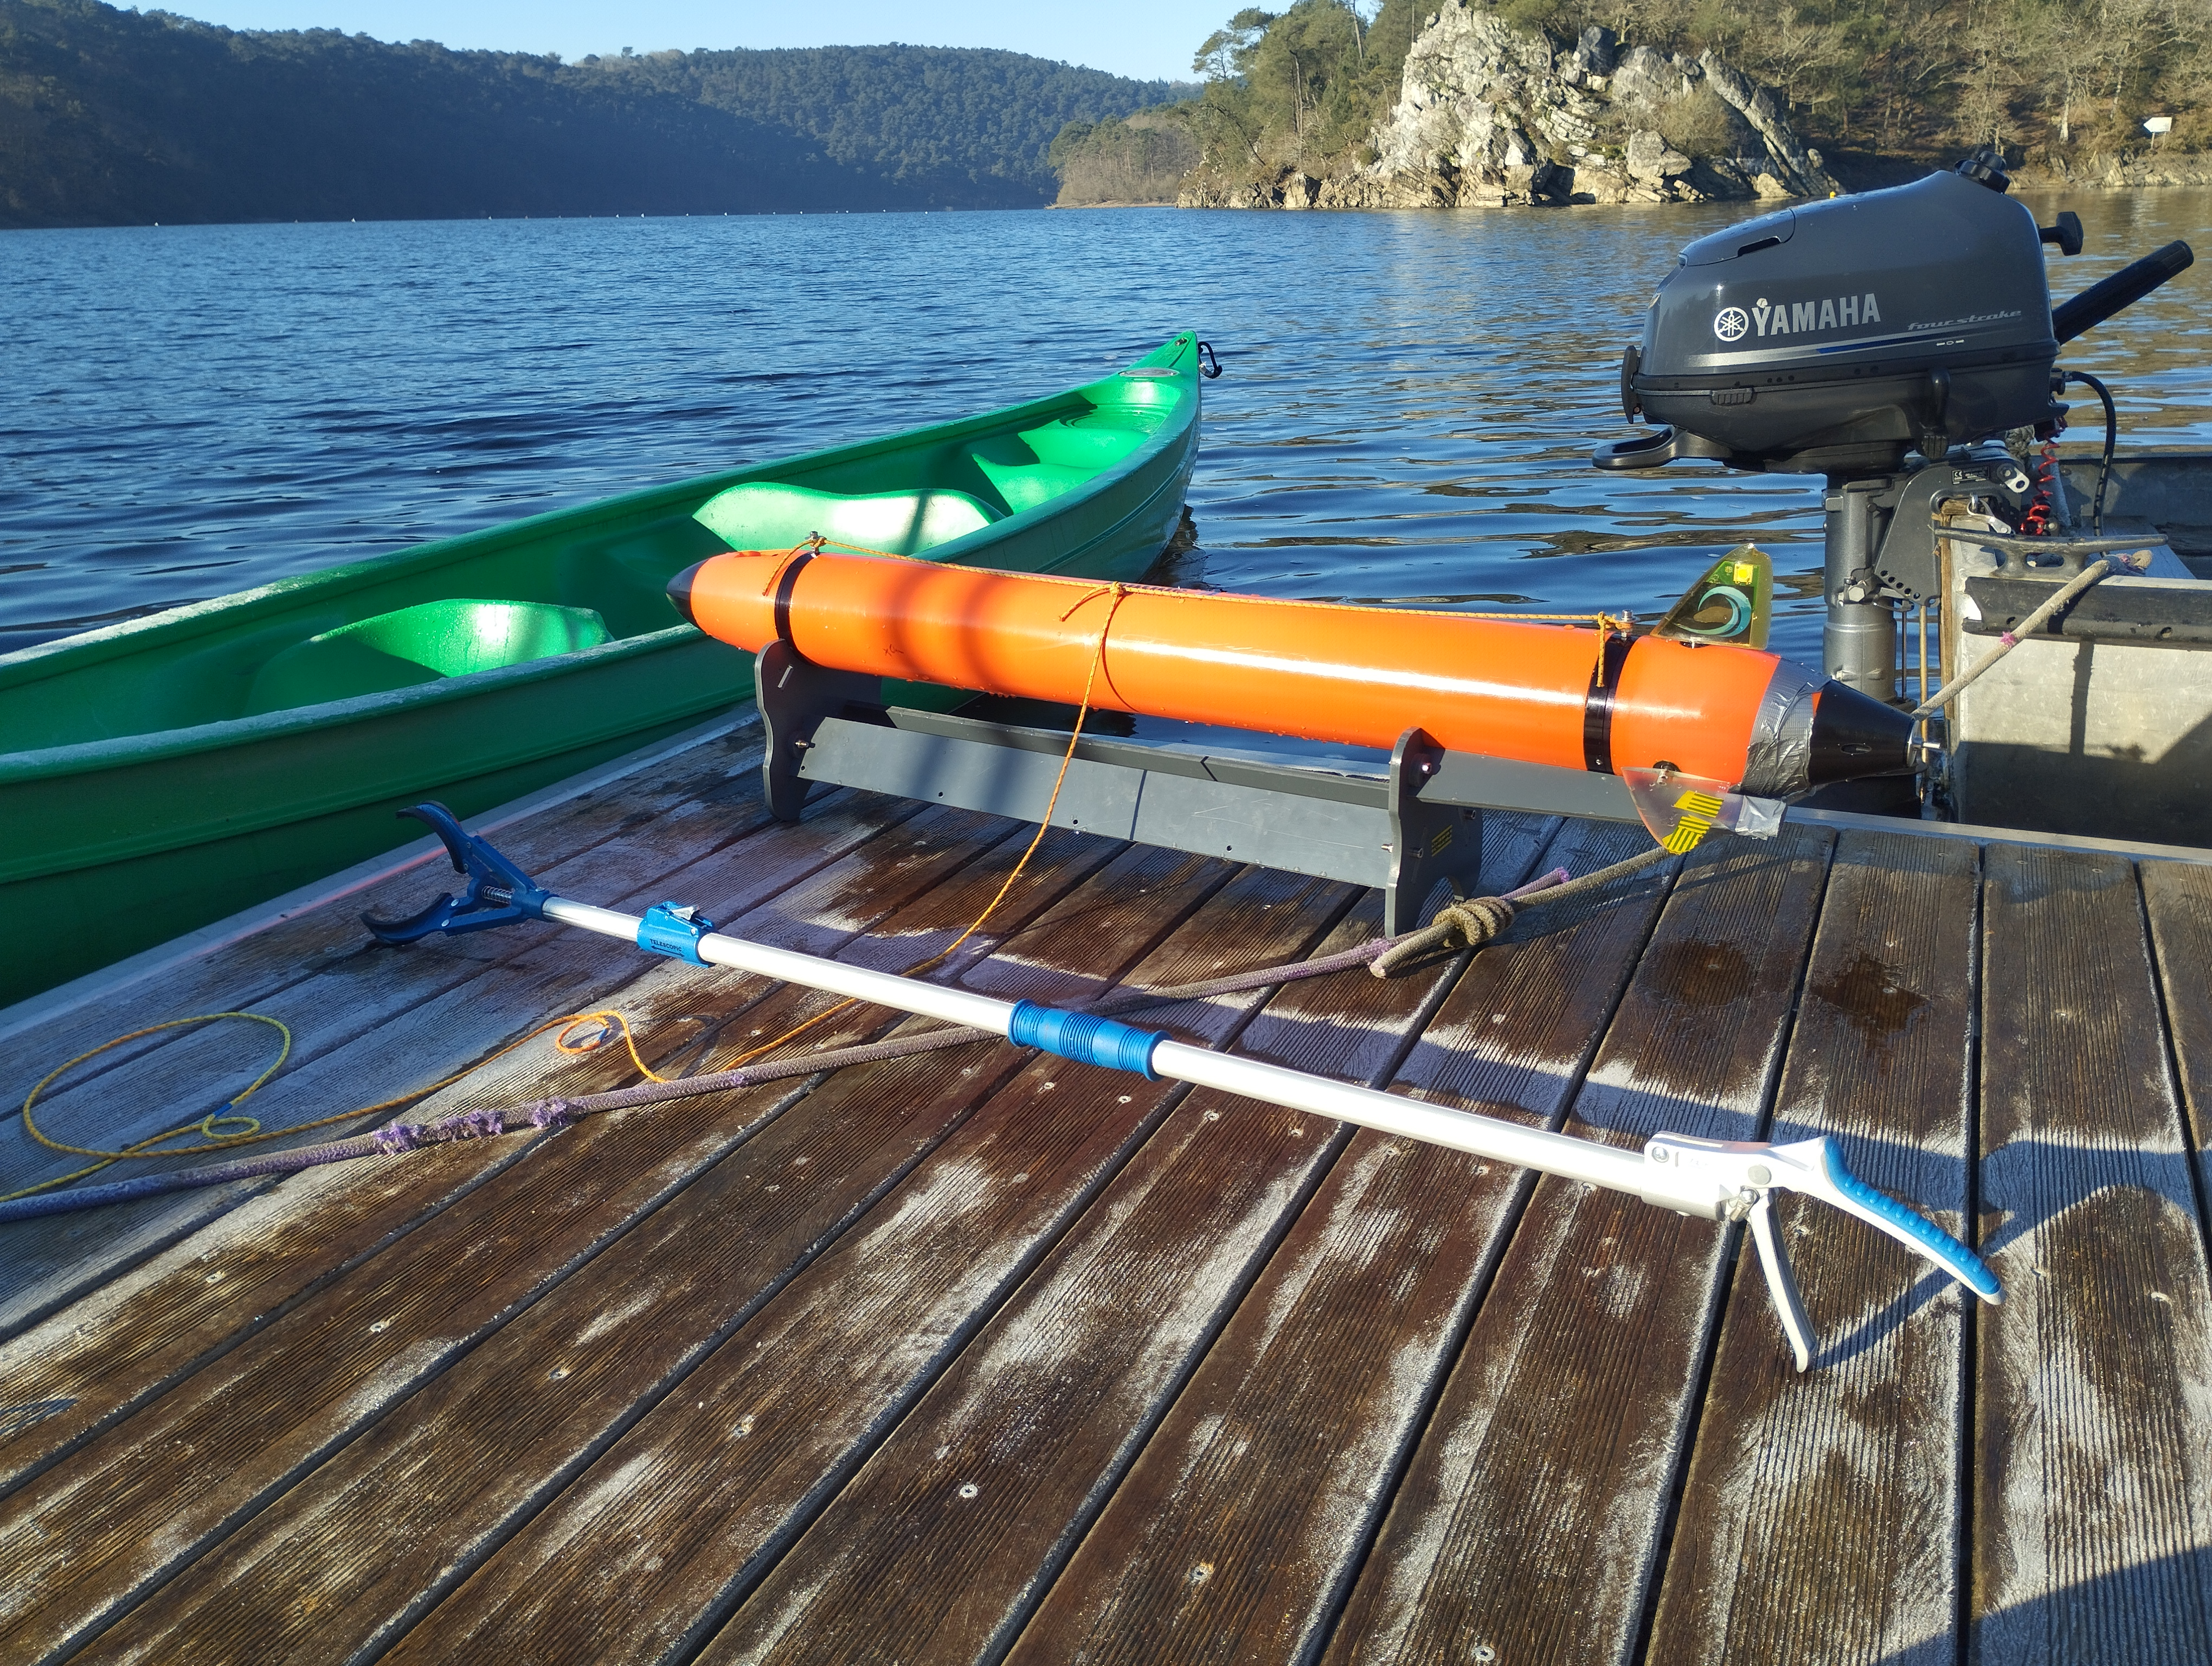
\includegraphics[width=\textwidth,trim={0 16cm 0 20cm},clip]{imgs/riptide_pontoon_2.jpg}
                            \subcaption{Riptide on pontoon}
                        \end{subfigure}
                        \caption{Guerlédan trials}
                    \end{figure}
                \end{minipage}
            \end{frame}

        \subsection{Depth controller trial}

            \begin{frame}{Depth Controller - Bloc diagram}
                \centering
                \begin{figure}
                    \begin{tikzpicture}[
                        input/.style={->,>=latex,thick,decorate,
                        decoration={snake,amplitude=.4mm,segment length=2mm,post length=2mm}},
                        block/.style={draw,font=\small,thick,
                            minimum width={2cm},minimum height={1.5cm}}]

                        \onslide<1-> \node[block,rectangle,align=center] (n3) {AUV};

                        \onslide<2->{
                            \node[block,circle,left=of n3] (n2) {Controller};
                            \coordinate (twist) at (n2.west);
                            \foreach \i/\a/\s in {0/37.5/-2.4,1/12.5/-3,2/-12.5/-3,3/-37.5/-2.5} {
                                \draw[thick,->,>=latex,Dandelion] (n2.\a) to node[near end,xshift=\s*1mm,yshift=1.5mm] {$u_\i$} ([yshift=0.6cm -\i * 0.4 cm]n3.west);
                            }
                        }

                        \onslide<3->{
                            \node[block,circle,left=of n2,align=center] (n1) {Depth\\controller};
                            \draw[thick,->,>=latex,RoyalBlue] (n1) to node[midway,above] {$\mathbf{v}$} node[midway,below] {$\mathbf{w}$} (twist);
                        }

                        \onslide<4->{
                            \coordinate(t) at ([shift=({145:2 cm})]n1);
                            \draw[input,ForestGreen] (t) -- node[midway,below left,ForestGreen] {$\mathbf{d}$} (n1.145);
                        }

                        \onslide<5->{
                            \node[yshift=-0.8cm,RoyalPurple] (f) at (n2.south) {$\mathbf{d}$, $\mathbf{pitch}$};
                            \draw[thick,RoyalPurple,->,>=latex] (n3.south) |- ($(f)+(0,0.3)$) -| (n1.south);
                        }
                    \end{tikzpicture}
                    \caption{Depth controller - Closed-loop block diagram}
                \end{figure}
            \end{frame}

            \begin{frame}{Mission description}
                \sisetup{input-digits = 0123456789\infty}
                \centering
                \begin{minipage}[c]{0.4\textwidth}
                    \centering
                    \begin{table}
                        \begin{tabular}[t]{ccc}
                            \toprule
                            State & Depth & Duration \\
                            \midrule
                            $q_0$ & $\qty{0}{\m}$ & $\qty{\infty}{\s}$ \\
                            % \AC{red} \hdashline[.6pt/1.2pt] \EAC
                            $q_1$ & $\qty{2}{\m}$ & $\qty{10}{\s}$ \\
                            $q_2$ & $\qty{1}{\m}$ & $\qty{10}{\s}$ \\
                            $q_3$ & $\qty{2}{\m}$ & $\qty{10}{\s}$ \\
                            \bottomrule
                        \end{tabular}
                        \caption{States description}
                    \end{table}
                \end{minipage}
                \hfill
                \begin{minipage}[c]{0.55\textwidth}
                    \begin{figure}[\textwidth]
                        \centering
                        \begin{tikzpicture}[node distance=2cm,on grid,auto]
                            \node[state, initial, accepting] (q0) {$q_0$};
                            \node[state, above right of=q0] (q1) {$q_1$};
                            \node[state, below right of=q0] (q3) {$q_3$};
                            \node[state, below right of=q1] (q2) {$q_2$};
                            
                            \draw[->,>=latex]
                                (q0) edge node[midway, above left] {\color{RubineRed}{trigger}} (q1)
                                (q1) edge node[midway, above right] {$d=\qty{10}{\s}$} (q2)
                                (q2) edge node[midway, below right] {$d=\qty{10}{\s}$} (q3)
                                (q3) edge node[midway, below left] {$d=\qty{10}{\s}$} (q0);
                        \end{tikzpicture}
                        \caption{FSM of the mission}
                    \end{figure}
                \end{minipage}
            \end{frame}

            \begin{frame}{Simulation}
                \centering
                \begin{minipage}[c]{0.95\textwidth}
                    \begin{figure}
                        \href{run:simulation.mkv?autostart&loop}{\includegraphics[width=\textwidth]{build/imgs/videos/simulation}}
                        \caption{Mission simulation}
                    \end{figure}
                \end{minipage}
            \end{frame}

            \begin{frame}{Simulation Data}
                \centering
                \begin{figure}
                    \centering
                    \begin{tikzpicture}
                        \begin{axis}[
                                mplot,
                                name=depth,
                                xlabel=Time,
                                ylabel=Depth,
                                x unit=\si{\s},
                                y unit=\si{\m},
                            ]
                            \addplot[RoyalBlue] table [x expr={\fpeval{\thisrow{pressure_stamp} - 1681203552.}}, y=depth, col sep=comma] {data/simulation.csv};
                        \end{axis}

                        \begin{axis}[
                                mplot,
                                name=fins,
                                at=(depth.right of north east), anchor=left of north west,
                                xshift=.25cm,
                                xlabel=Time,
                                ylabel=Fin angle,
                                x unit=\si{\s},
                                y unit=\si{\radian},
                            ]
                            \addplot[Dandelion] table [x expr={\fpeval{\thisrow{time} - 1681203552.}}, y=p_fin, col sep=comma] {data/simulation.csv};
                            \addplot[RubineRed] table [x expr={\fpeval{\thisrow{time} - 1681203552.}}, y=s_fin, col sep=comma] {data/simulation.csv};
                        \end{axis}

                        \begin{axis}[
                                mplot,
                                name=pressure,
                                at=(depth.below south west), anchor=above north west,
                                xlabel=Time,
                                ylabel=Pressure,
                                x unit=\si{\s},
                                y unit=\si{\pascal},
                            ]
                            \addplot[RoyalPurple] table [x expr={\fpeval{\thisrow{pressure_stamp} - 1681203552.}}, y=pressure, col sep=comma] {data/simulation.csv};
                        \end{axis}

                        \begin{axis}[
                                mplot,
                                name=pitch,
                                at=(fins.below south west), anchor=above north west,
                                xlabel=Time,
                                ylabel=Pitch,
                                x unit=\si{\s},
                                y unit=\si{\deg},
                            ]
                            \addplot[ForestGreen] table [x expr={\fpeval{\thisrow{time} - 1681203552.}}, y=/riptide_1/imu_broadcaster/imu_status/orientation/pitch_deg, col sep=comma] {data/simulation.csv};
                        \end{axis}
                    \end{tikzpicture}
                    \caption{Mission simulation}
                \end{figure}
            \end{frame}

            \begin{frame}{Mission Data}
                \centering
                \begin{figure}
                    \centering
                    \begin{tikzpicture}
                        \begin{axis}[
                                mplot,
                                name=depth,
                                xlabel=Time,
                                ylabel=Depth,
                                x unit=\si{\s},
                                y unit=\si{\m},
                            ]
                            \addplot[RoyalBlue] table [x expr={\fpeval{\thisrow{stamp} - 1684869329.}}, y=depth, col sep=comma] {data/trial/pressure.csv};
                        \end{axis}

                        \begin{axis}[
                                mplot,
                                name=fins,
                                at=(depth.right of north east), anchor=left of north west,
                                xshift=.25cm,
                                xlabel=Time,
                                ylabel=Fin angle,
                                x unit=\si{\s},
                                y unit=\si{\radian},
                            ]
                            \addplot[Dandelion] table [x expr={\fpeval{\thisrow{stamp} - 1684869329.}}, y=p_fin, col sep=comma] {data/trial/actuators.csv};
                            \addplot[RubineRed] table [x expr={\fpeval{\thisrow{stamp} - 1684869329.}}, y=s_fin, col sep=comma] {data/trial/actuators.csv};
                        \end{axis}

                        \begin{axis}[
                                mplot,
                                name=pressure,
                                at=(depth.below south west), anchor=above north west,
                                xlabel=Time,
                                ylabel=Pressure,
                                x unit=\si{\s},
                                y unit=\si{\pascal},
                            ]
                            \addplot[RoyalPurple] table [x expr={\fpeval{\thisrow{stamp} - 1684869329.}}, y=pressure, col sep=comma] {data/trial/pressure.csv};
                        \end{axis}

                        \begin{axis}[
                                mplot,
                                name=pitch,
                                at=(fins.below south west), anchor=above north west,
                                xlabel=Time,
                                ylabel=Pitch,
                                x unit=\si{\s},
                                y unit=\si{\deg},
                            ]
                            \addplot[ForestGreen] table [x expr={\fpeval{\thisrow{stamp} - 1684869329.}}, y expr={\fpeval{\thisrow{pitch} * 180./3.1415}}, col sep=comma] {data/trial/imu.csv};
                        \end{axis}
                    \end{tikzpicture}
                    \caption{Real mission data}
                \end{figure}
            \end{frame}

        % \subsection{Log controller software architecture}

        %     \begin{frame}{Log Controller - Bloc diagram}
        %         \centering
        %         \begin{figure}
        %             \begin{tikzpicture}[
        %                 input/.style={->,>=latex,thick,decorate,
        %                 decoration={snake,amplitude=.4mm,segment length=2mm,post length=2mm}},
        %                 block/.style={draw,font=\small,thick,
        %                     minimum width={2cm},minimum height={1.5cm}}]

        %                 \onslide<+-> \node[block,rectangle,align=center] (n3) {AUV};

        %                 \onslide<+->{
        %                     \node[block,circle,left=of n3] (n2) {Controller};
        %                     \coordinate (twist) at (n2.west);
        %                     \foreach \i/\a/\s in {0/37.5/-2.4,1/12.5/-3,2/-12.5/-3,3/-37.5/-2.5} {
        %                         \draw[thick,->,>=latex,Dandelion] (n2.\a) to node[near end,xshift=\s*1mm,yshift=1.5mm] {$u_\i$} ([yshift=0.6cm -\i * 0.4 cm]n3.west);
        %                     }
        %                 }

        %                 \onslide<+->{
        %                     \node[block,circle,left=of n2,align=center] (n1) {Log\\controller};
        %                     \draw[thick,->,>=latex,RoyalBlue] (n1) to node[midway,above] {$\mathbf{v}$} node[midway,below] {$\mathbf{w}$} (twist);
        %                 }

        %                 % Inputs
        %                 \onslide<+>{
        %                     \coordinate[above=of n1.100] (u);
        %                     \draw[input,red] (u) -- node[midway,left,red] {$\mathbf{R_u}$} (n1.100);
        %                     \coordinate[above=of n1.80] (v);
        %                     \draw[input,ForestGreen] (v) -- node[midway,right,ForestGreen] {$\mathbf{R_v}$} (n1.80);
        %                 }

        %                 \onslide<.->{
        %                     \coordinate(t) at ([shift=({145:2 cm})]n1);
        %                     \draw[input,RubineRed] (t) -- node[midway,below left,RubineRed] {$\mathbf{t}$} (n1.145);
        %                 }

        %                 \onslide<+->{
        %                     \node[yshift=-0.8cm,RoyalPurple] (Ru) at (n2.south) {$\mathbf{R_u}$};
        %                     \draw[thick,RoyalPurple,->,>=latex] (n3.south) |- ($(Ru)+(0,0.3)$) -| (n1.south);
        %                     \coordinate[above=of n1.90] (v);
        %                     \draw[input,ForestGreen] (v) -- node[midway,right,ForestGreen] {$\mathbf{R_v}$} (n1.90);
        %                 }
        %             \end{tikzpicture}
        %             \caption{Log controller -
        %                 \only<1-4>{Open-loop}\only<5->{Closed-loop} block diagram 
        %             }
        %         \end{figure}
        %     \end{frame}
        
        % \subsection{Orthogonal controller software architecture}
        
        %     \begin{frame}{Orthogonal Controller - Bloc diagram}
        %         \centering
        %         \begin{figure}
        %             \begin{tikzpicture}[
        %                 input/.style={->,>=latex,thick,decorate,
        %                 decoration={snake,amplitude=.4mm,segment length=2mm,post length=2mm}},
        %                 block/.style={draw,font=\small,thick,
        %                     minimum width={2cm},minimum height={1.5cm}}]

        %                 \onslide<+-> \node[block,rectangle,align=center] (n3) {AUV};

        %                 \onslide<+->{
        %                     \node[block,circle,left=of n3] (n2) {Controller};
        %                     \coordinate (twist) at (n2.west);
        %                     \foreach \i/\a/\s in {0/37.5/-2.4,1/12.5/-3,2/-12.5/-3,3/-37.5/-2.5} {
        %                         \draw[thick,->,>=latex,Dandelion] (n2.\a) to node[near end,xshift=\s*1mm,yshift=1.5mm] {$u_\i$} ([yshift=0.6cm -\i * 0.4 cm]n3.west);
        %                     }
        %                 }

        %                 \onslide<+->{
        %                     \node[block,circle,left=of n2,align=center] (n1) {Orthogonal\\controller};
        %                     \draw[thick,->,>=latex,RoyalBlue] (n1) to node[midway,above] {$\mathbf{v}$} node[midway,below] {$\mathbf{w}$} (twist);
        %                 }

        %                 % Inputs
        %                 \onslide<+->{
        %                     \coordinate[above=of n1.100] (u);
        %                     \draw[input,red] (u) -- node[midway,left,red] {$\mathbf{u}$} (n1.100);
        %                     \coordinate[above=of n1.80] (v);
        %                     \draw[input,ForestGreen] (v) -- node[midway,right,ForestGreen] {$\mathbf{v}$} (n1.80);
        %                     \coordinate(t) at ([shift=({145:2 cm})]n1);
        %                     \draw[input,RubineRed] (t) -- node[midway,below left,RubineRed] {$\mathbf{t}$} (n1.145);
        %                 }

        %                 \onslide<+->{
        %                     \node[yshift=-0.8cm,RoyalPurple] (Ru) at (n2.south) {$\mathbf{w}$};
        %                     \draw[thick,RoyalPurple,->,>=latex] (n3.south) |- ($(Ru)+(0,0.3)$) -| (n1.south);
        %                 }
        %             \end{tikzpicture}
        %             \caption{Orthogonal controller - Closed-loop block diagram 
        %             }
        %         \end{figure}
        %     \end{frame}
    
    \section{State estimation}

        \subsection{Geometric contractors}
            
            \begin{frame}{Geometric contractors}
                \begin{minipage}[t]{.45\textwidth}
                    \begin{block}{Geometric contractors}
                        \vspace{2.5mm}
                        \begin{itemize}
                            \item<1-> Contractors based on geometrical constraints
                            \item<2-> Usefull in localization
                        \end{itemize}
                    \end{block}
                    \begin{exampleblock}<3->{Example}
                        \begin{itemize}[<+->]
                            \item<3-> CtcCross
                            \item<4-> CtcVisible
                        \end{itemize}
                    \end{exampleblock}
                \end{minipage}%
                \hfill
                \begin{minipage}[t]{.5\textwidth}
                    \begin{figure}
                        \begin{overprint}
                            \onslide<3>\centerline{\input{imgs/sepcross_segment.pgf}}
                            \onslide<4>\centerline{\input{imgs/sepvisible_segment.pgf}}
                        \end{overprint}
                        \vspace{-8mm}
                        \begin{overprint}
                            \onslide<3>\caption{Cross separator}
                            \onslide<4>\caption{Visibility separator}
                        \end{overprint}
                    \end{figure}
                \end{minipage}
            \end{frame}

            \begin{frame}{Localization}
                \begin{minipage}[c]{.55\textwidth}
                    \begin{alertblock}{Constraints}
                        \vspace{0.25cm}
                        \begin{itemize}
                            \item<2-> The robot is in the pool
                            \item<3-> There is at least $d$ meters in the echosounder's direction
                        \end{itemize}
                    \end{alertblock}
                    \onslide<4->{
                        \begin{figure}
                            \resizebox*{!}{.6\textwidth}{
                                \input{imgs/robot_zoom.pgf}
                            }
                            \caption{Uncertain area}
                        \end{figure}
                    }
                \end{minipage}%
                \hfill
                \begin{minipage}[c]{.45\textwidth}
                    \centering
                    \begin{figure}
                        \begin{overprint}
                            \onslide<1>\centerline{\input{imgs/robot_unknown.pgf}}
                            \onslide<2>\centerline{\input{imgs/robot_pool.pgf}}
                            \onslide<3->\centerline{\input{imgs/robot_echosounder.pgf}}
                        \end{overprint}
                        \caption{\only<1>{Unknown localization}\only<2>{Robot is in the pool}\only<3->{Distance measurement}}
                   \end{figure}
                \end{minipage}
            \end{frame}

    \section{Conclusion}

        % \begin{frame}{Conclusion}
        %     \centering
        %     \begin{minipage}{0.8\textwidth}
        %         \begin{block}{Log control}
        %             \vspace*{.25cm}
        %             \begin{itemize}
        %                 \item Simple and elegant control law
        %                 \item Fastest reorientation along a geodesic in $SO(3)$
        %                 \item Applicable in orientation control of various robots 
        %                 \item Need a complete knowledge of $\mathbf{R}$
        %             \end{itemize}
        %         \end{block}
        %         \begin{block}{Outlook}
        %             \begin{itemize}
        %                 \item Fix Riptide's hardware
        %                 \item Field experiments on Riptide
        %             \end{itemize}
        %         \end{block}
        %     \end{minipage}
        % \end{frame}

    \appendix

        \begin{frame}[standout]
            Questions?
        \end{frame}

        \begin{frame}{Lie algebra vs Lie group}
            \begin{figure}
                \begin{tikzpicture}
                    % Lie algebra
                    \begin{scope}[xshift=-3cm]
                        \draw[black,inner color=gray!10, outer color=gray!40] (-1.5,1.5) rectangle (1.5,-1.5);
                        \coordinate (I) at (-1.1,-1.1);
                        \coordinate (R1) at (0.6,1.1);
                        \node[RoyalPurple] at (R1) {$\bullet$} node[RoyalPurple] at (R1) [yshift=-0.5cm,xshift=-0.6cm] {\footnotesize$\mathbf{w}\wedge\left(\begin{smallmatrix}0&-w_z&w_y\\w_z&0&-w_x\\-w_y&w_x&0\end{smallmatrix}\right)$};
                        \node[RoyalBlue] at (I) {$\bullet$} node[RoyalBlue] at (I) [above,xshift=0.5cm] {\footnotesize$\mathbf{a}\wedge\left(\begin{smallmatrix}0&0&0\\0&0&0\\0&0&0\end{smallmatrix}\right)$};
                        \coordinate (LAr) at (1.5,0);
                        \coordinate (LAb) at (-0.75,-1.5);
                    \end{scope}

                    % Lie group
                    \begin{scope}[scale=0.9,xshift=3cm]
                        \shade[ball color = gray!40, opacity = 0.4] (0,0) circle (2cm);
                        \draw[thick] (-2,0) arc (180:360:2 and 0.6) coordinate[pos=0.3] (I);
                        \draw[dashed] (2,0) arc (0:180:2 and 0.6);
                        \draw[thick] (0,0) circle (2cm);
                        \coordinate (R1) at (-0.6,1.1);
                        \node[RoyalPurple] at (R1) {$\bullet$} node[RoyalPurple] at (R1) [yshift=-0.5cm,xshift=0.6cm] {\footnotesize$\mathbf{R}=exp\left(\begin{smallmatrix}0&-w_z&w_y\\w_z&0&-w_x\\-w_y&w_x&0\end{smallmatrix}\right)$};
                        \node[RoyalBlue] at (I) {$\bullet$} node[RoyalBlue] at (I) [below,xshift=0.5cm] {\footnotesize$\mathbf{I}=exp\left(\begin{smallmatrix}0&0&0\\0&0&0\\0&0&0\end{smallmatrix}\right)$};
                        \coordinate (LGl) at (-2,0);
                        \coordinate (LGb) at (0.75,-2);
                    \end{scope}

                    \begin{scope}[scale=0.18,xshift=-6cm,yshift=-20cm]
                        % The axes
                        \draw[->,>=latex] (xyz cs:x=-2) -- (xyz cs:x=10) node[above] {$x$};
                        \draw[->,>=latex] (xyz cs:y=-2) -- (xyz cs:y=10) node[right] {$z$};
                        \draw[->,>=latex] (xyz cs:z=-10) -- (xyz cs:z=10) node[above] {$y$};

                        % Thin ticks
                        \foreach \coo in {-2,0,...,8} {
                            \draw (\coo,-4pt) -- (\coo,4pt);
                            \draw (-4pt,\coo) -- (4pt,\coo);
                        }
                        \foreach \coo in {-10,-8,...,8} {
                            \draw (xyz cs:y=-0.15pt,z=\coo) -- (xyz cs:y=0.15pt,z=\coo);
                        }
                        
                        % Dashed lines for the points P, Q
                        \draw[dashed] (xyz cs:z=-5) -- +(0,7) coordinate (u) -- (xyz cs:y=7) -- +(5,0) -- 
                            ++(xyz cs:x=5,z=-5) coordinate (v) --+(0,-7) coordinate (w) -- cycle;
                        \draw[dashed] (u) -- (v);
                        \draw[dashed] (5,7) -- (5,0) -- (w);

                        % Dots and labels for P, Q
                        \coordinate (I) at (0,0);
                        \node[RoyalBlue] at (I) {$\bullet$} node[RoyalBlue] at (I) [above,xshift=-0.6cm] {\footnotesize$\mathbf{a}\left(\begin{smallmatrix}0\\0\\0\end{smallmatrix}\right)$};
                        \node[RoyalPurple] at (v) {$\bullet$} node[RoyalPurple] at (v) [right] {\footnotesize$\mathbf{w}\left(\begin{smallmatrix}w_x\\w_y\\w_z\end{smallmatrix}\right)$};

                        \coordinate (Rl) at (-6,2);
                        \coordinate (Rr) at (12,2);
                    \end{scope}

                    \draw[->,>=latex] ([xshift=.25cm,yshift=.25cm]LAr) to [bend left] node [midway,above] {$exp$} ([xshift=-.25cm,yshift=.25cm]LGl);
                    \draw[->,>=latex] ([xshift=-.25cm,yshift=-.25cm]LGl) to [bend left] node [midway,below] {$log$} ([xshift=.25cm,yshift=-.25cm]LAr);
                    
                    \draw[->,>=latex] ([xshift=.25cm,yshift=-.25cm]LAb) to [bend right] node [midway,above right] {$\vee$} ([xshift=-.25cm,yshift=.25cm]Rl);
                    \draw[->,>=latex] ([xshift=-.25cm,yshift=-.25cm]Rl) to [bend left] node [midway,below left] {$\wedge$} ([xshift=-.25cm,yshift=-.25cm]LAb);
                    
                    \draw[->,>=latex] ([xshift=.25cm,yshift=.25cm]Rr) to [bend right] node [midway,above left] {$Exp$} ([xshift=-.25cm,yshift=-.25cm]LGb);
                    \draw[->,>=latex] ([xshift=.25cm,yshift=-.25cm]LGb) to [bend left] node [midway,below right] {$Log$} ([xshift=.25cm,yshift=-.25cm]Rr);

                \end{tikzpicture}
                \caption{Relationship between Lie algebra and Lie group}
            \end{figure}
        \end{frame}

        % \begin{frame}{Control}
        %     \centering
        %     \begin{minipage}{0.7\textwidth}
        %         \begin{block}{Control inputs}
        %             \centering
        %             Controlled physical quantites are linear acceleration $\mathbf{a_r}$ and angular velocity $\mathbf{\omega_r}$
        %         \end{block}
        %         \begin{block}{State Equation}
        %             \begin{eqnarray}
        %                 \left\{
        %                     \begin{array}{rcl}
        %                         \dot{\mathbf{p}} & = & \mathbf{R} \cdot \mathbf{v_r} \\
        %                         \dot{\mathbf{R}} & = & \mathbf{R} \cdot (\mathbf{\omega_r} \wedge) \\
        %                         \dot{\mathbf{v_r}} & = & \mathbf{R}^T \cdot g(\mathbf{p}) + \mathbf{a_r} - \mathbf{\omega_r} \wedge \mathbf{v_r}
        %                     \end{array}
        %                 \right.
        %             \end{eqnarray}
        %         \end{block}
        %     \end{minipage}
        % \end{frame}


        % \begin{frame}{Torpedo model}
        %     \centering
        %     \begin{minipage}{0.7\textwidth}
        %         \begin{block}{Torpedo assumptions}
        %             The following statements are equivalent
        %             \begin{itemize}
        %                 \item No side slip effect \\
        %                 \item No lateral speed
        %                 \item Velocity along the $\mathnormal{x}$ axis \\
        %             \end{itemize}
        %         \end{block}
        %         \begin{block}{Torpedo velocity}
        %             \begin{equation}
        %                 \mathbf{v_r} = (v_r, 0, 0)^T
        %             \end{equation}
        %         \end{block}
        %     \end{minipage}
        % \end{frame}

        % \begin{frame}{State Equation}
        %     \centering
        %     \begin{minipage}{0.7\textwidth}
        %         \begin{block}{AUV state}
        %             The state of the AUV is denoted by $\mathbf{X} = (\mathbf{p}, \mathbf{v_r}, \mathbf{R})$, where:
        %             \begin{itemize}
        %                 \item $\mathbf{p}$ is the position of the AUV \\
        %                 \item $\mathbf{v_r}$ is the velocity of the AUV in its frame \\
        %                 \item $\mathbf{R}$ is the rotation matrix between the world and the AUV \\
        %             \end{itemize}
        %         \end{block}
        %         \begin{block}{State Equation}
        %             \begin{eqnarray}
        %                 \left\{
        %                     \begin{array}{rcl}
        %                         \dot{\mathbf{p}} & = & \mathbf{R} \cdot \mathbf{v_r} \\
        %                         \dot{\mathbf{R}} & = & \mathbf{R} \cdot (\mathbf{\omega_r} \wedge) \\
        %                         \dot{\mathbf{v_r}} & = & \mathbf{R}^T \cdot g(\mathbf{p}) + \mathbf{a_r}
        %                     \end{array}
        %                 \right.
        %             \end{eqnarray}
        %         \end{block}
        %     \end{minipage}
        % \end{frame}

        % \begin{frame}{Inputs}
        %     \centering
        %     \begin{minipage}{0.7\textwidth}
        %         \begin{block}{Inputs}
        %             \centering
        %             Input vector of the system is $\mathbf{u} = (u_0, u_1, u_2, u_3)^T$, where:
        %             \begin{itemize}
        %                 \item $u_0$: thruster velocity \\
        %                 \item $u_1, u_2, u_3$: fin angles
        %             \end{itemize}
        %         \end{block}
        %     \end{minipage}
        % \end{frame}

        % \begin{frame}{Linear acceleration}
        %     \centering
        %     \begin{minipage}{0.7\textwidth}
        %         \begin{block}{Assumptions}
        %             \vspace{0.2cm}
        %             \begin{itemize}
        %                 \item Quadratic thrust with velocity
        %                 \item Quadratic drag with velocity
        %             \end{itemize}
        %         \end{block}
        %         \begin{block}{Linear acceleration}
        %             \begin{equation}
        %                 \mathbf{a_r} = \underbrace{p_1 \cdot \left(\begin{smallmatrix}u_0 \\ 0 \\ 0 \end{smallmatrix}\right)^2}_{thrust} - \underbrace{p_2 \cdot \mathbf{v_r} \cdot |\mathbf{v_r}|}_{drag}
        %             \end{equation}
        %         \end{block}
        %     \end{minipage}
        % \end{frame}

        % \begin{frame}{Angular velocity}
        %     \centering
        %     \begin{minipage}{0.8\textwidth}
        %         \begin{block}{Assumptions}
        %             \vspace{0.2cm}
        %             \begin{itemize}
        %                 \item Fin's drag negligible compared to the AUV drag
        %                 \item Fin's lift used to control the AUV
        %                 \item Direct response between the fin's angle and the angular velocity
        %             \end{itemize}
        %         \end{block}
        %         \begin{block}{Angular velocity}
        %             \begin{equation}
        %                 \mathbf{\omega_r} = v_r^{\color{red}{2}} \cdot 
        %                     \underbrace{
        %                         \left(
        %                         \begin{smallmatrix}
        %                             -p_3 & -p_3 & -p_3 \\
        %                             0 & p_4 \cdot sin(\frac{2\pi}{3}) & -p_4 \cdot sin(\frac{2\pi}{3}) \\
        %                             p_4 & p_4 \cdot cos(\frac{2\pi}{3}) & p_4 \cdot cos(\frac{2\pi}{3})
        %                         \end{smallmatrix}
        %                         \right)
        %                     }_{\mathbf{B}(p_3, p_4)} \cdot \left(\begin{smallmatrix}u_1\\ u_2\\ u_3\end{smallmatrix}\right)
        %             \end{equation}
        %         \end{block}
        %     \end{minipage}
        % \end{frame}

        % \begin{frame}{Repartition matrix}
        %     \centering
        %     \begin{minipage}{0.8\textwidth}
        %         \begin{block}{Fin's lift}
        %             $\forall i \in \{0, 1, 2\}:$
        %             \begin{itemize}
        %                 \item Force $\mathbf{f_i} = \alpha \cdot u_i \cdot v^2 \cdot (0, 1, 0)^T$
        %                 \item Orientation $\mathbf{R_i} = \mathbf{R_x}\left(\frac{2i\pi}{3}\right)$
        %                 \item Center of pressure $\mathbf{q_i} = (\mathit{l_x}, 0, \mathit{l_z})^T$
        %                 \item Torque $\mathbf{\tau_i} = \mathbf{R_i} \cdot \mathbf{q} \wedge \mathbf{f_i}$
        %             \end{itemize}
        %         \end{block}
        %         \begin{block}{Angular velocity}
        %             \begin{equation}
        %                 \mathbf{\omega_r} = v_r^2 \cdot 
        %                     \underbrace{
        %                         \left(
        %                         \begin{smallmatrix}
        %                             -p_3 & -p_3 & -p_3 \\
        %                             0 & p_4 \cdot sin(\frac{2\pi}{3}) & -p_4 \cdot sin(\frac{2\pi}{3}) \\
        %                             p_4 & p_4 \cdot cos(\frac{2\pi}{3}) & p_4 \cdot cos(\frac{2\pi}{3})
        %                         \end{smallmatrix}
        %                         \right)
        %                     }_{\mathbf{B}(p_3, p_4)} \cdot \left(\begin{smallmatrix}u_1\\ u_2\\ u_3\end{smallmatrix}\right)
        %             \end{equation}
        %         \end{block}
        %     \end{minipage}
        % \end{frame}
    
\end{document}